%\chapter{Numerical Examples}
\chapter{実験・考察}

構成したSIBMを以下の実験環境(表\ref{table:sibm_env})で実装し、データの生成時間やデータベースシステムとのアクセス時間について考察を行う。

\begin{table}[h]
	\begin{center}
	\begin{tabular}{| l  p{45mm} |}
		\hline
		\rowstyle{\bfseries}
		実験環境 & \\
		\hline
		Operation System & Windows 8.1 Pro 64 bits \\
		CPU & Intel core i7 3770, 4 cores 8 thread @ 3.4Ghz (Boostable up to 3.9Ghz)
		\\
		RAM & 16GB \\
		Storage & HDD \\
		Java & 1.7.0\_71 (64 bits) \\
		Apache Jena & 2.12.1 \\
		SIBM & v0.9 build 20150129 \\
		\hline
	\end{tabular}
	\caption{実験環境}
	\label{table:sibm_env}
	\end{center}
\end{table}

SIBMを用いて生成したデータが図\ref{fig:sibm_sample}のような形になる。
	
\begin{figure}[h!]
	\lstinputlisting{./sample/sample.txt}
  	\caption{実装例}
  	\label{fig:sibm_sample}
\end{figure}

大数の避難場所情報を生成する場合、かかった時間やデータ量などの情報が表\ref{table:sibm_time_table}のようになる。

\begin{table}[h!]
	\begin{center}
	\begin{tabular}{| r | r | r | r | r | r |}
		\hline
		\rowstyle{\bfseries}
		避難場所数 & 生成時間(ms) & 関係者数 & トリプル数 & 挿入時間(ms) & サイズ(MB) \\
		\hline
		5 & 3373 & 1455 & 20409 & 3807 & 203.87 \\
		\hline
		10 & 4779 & 3018 & 42304 & 3669 & 205.57 \\
		\hline
		20 & 6783 & 6082 & 85482 & 5588 & 223.91 \\
		\hline
		50 & 7603 & 12645 & 177991 & 8312 & 296.59 \\
		\hline
		100 & 6591 & 24751 & 348443 & 12662 & 379.90 \\
		\hline
		200 & 10363 & 53719 & 755895 & 22522 & 625.34 \\
		\hline
		350 & 24708 & 112888 & 1584015 & 43468 & 1127.90 \\
		\hline
		500 & 30228 & 152903 & 2148284 & 55275 & 1456.53 \\
		\hline
		700 & 42229 & 220201 & 3091954 & 77798 & 2004.87 \\
		\hline
	\end{tabular}
	\caption{避難場所数に対する生成時間}
	\label{table:sibm_time_table}
	\end{center}
\end{table}

図\ref{fig:sibm_data_time}でわかるように、避難場所数が生成時間や人数・トリプル数と比例関係が確認できる。
また、Jena/TDBデータベースでは、挿入するデータに対するメタデータやインデクシングすることによる発生したデータが多い。
そのため、少量データに対してもデータベースサイズが192.0MBになることがわかる\footnote{https://jena.apache.org/documentation/tdb/architecture.html}。

\begin{figure}[t!]
 	\begin{center}
 		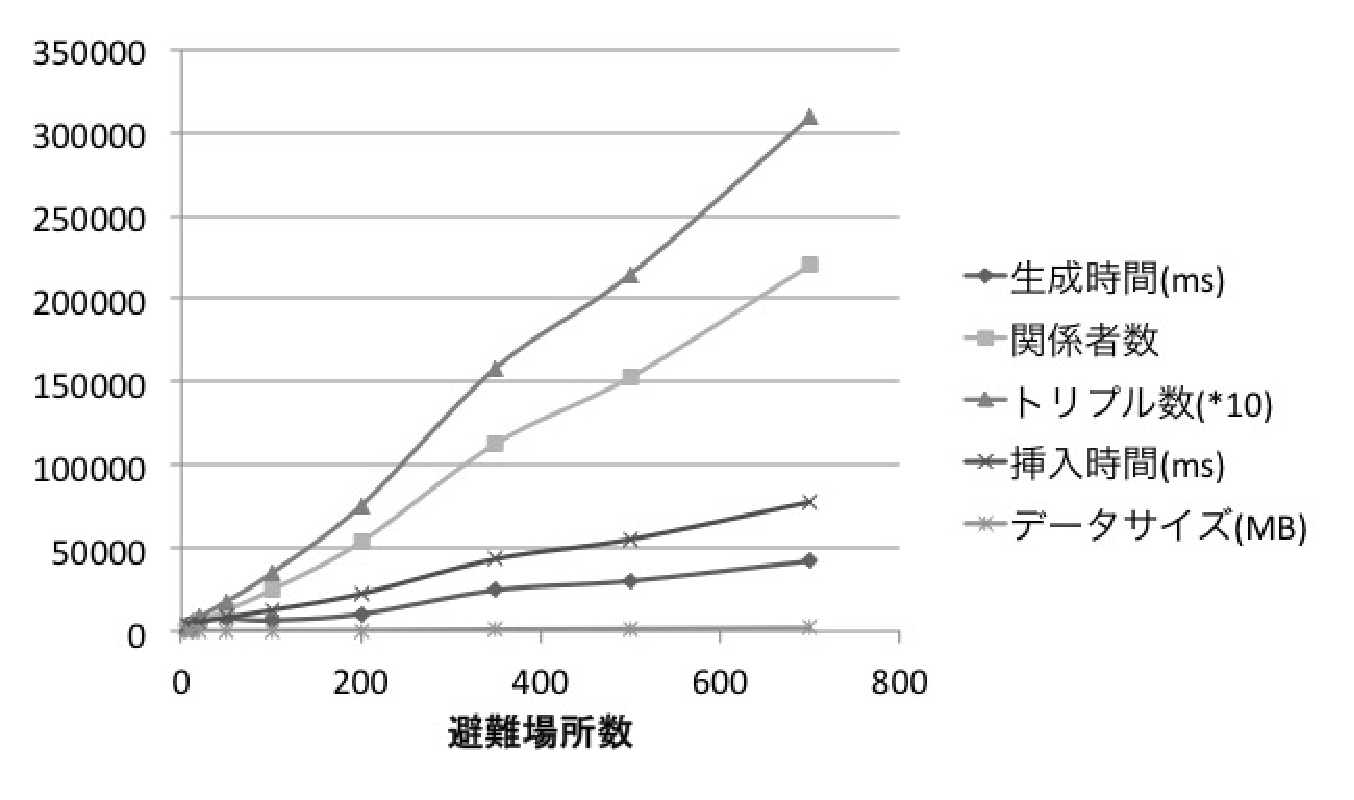
\includegraphics[width=120mm]{./images/test_chart1.eps}
 		\caption{生成・挿入時間とデータサイズ}
 		\label{fig:sibm_data_time}
 	\end{center}
\end{figure}

次に、生成したデータに対するクエリを行い、応答時間につい考察する。
なお、使用したクエリが\ref{appendix1}に説明する。また、Jena/TDBをデータストレージとして使用した。
実行時間とそれをグラフ化した物は以下の表\ref{table:sibm_query_time_1}、表\ref{table:sibm_query_time_2}
及び図\ref{fig:sibm_query_time}のようになる。

\begin{table}[h!]
	\begin{center}
	\begin{tabular}{| r | r | r | r | r | r | r |}
		\hline
		\rowstyle{\bfseries}
		避難場所数 & li\_q1 & li\_q2 & li\_q3 & li\_q4 &
		li\_q6 & li\_q7 \\
		\hline
		5 & 122 & 9 & 11 & 157 & 4 & 7 \\
		\hline
		10 & 203 & 9 & 12 & 240 & 4 & 6 \\
		\hline
		20 & 99 & 8 & 11 & 289 & 5 & 4 \\
		\hline
		50 & 96 & 9 & 14 & 375 & 6 & 4 \\
		\hline
		100 & 94 & 8 & 11 & 494 & 8 & 4 \\
		\hline
		200 & 97 & 9 & 11 & 799 & 13 & 4 \\
		\hline
		350 & 98 & 9 & 11 & 2157 & 91 & 4 \\
		\hline
		500 & 96 & 9 & 10 & 4576 & 32 & 4 \\
		\hline
		700 & 97 & 9 & 12 & 7779 & 82 & 4 \\
		\hline
	\end{tabular}
	\caption{クエリ時間(ms)(LUBMを参考したクエリセット)
	(「li」は「lubm\_insp」の略となる)}
	\label{table:sibm_query_time_1}
	\end{center}
\end{table}

\begin{table}[h!]
	\begin{center}
	\begin{tabular}{| r | r | r | r | r | r | r |}
		\hline
		\rowstyle{\bfseries}
		避難場所数 & label & age & family & gendet\_ext &
		storage & school \\
		\hline
		5 & 41 & 63 & 9 & 39 & 23 & 3 \\
		\hline
		10 & 46 & 73 & 9 & 39 & 4 & 3 \\
		\hline
		20 & 58 & 89 & 9 & 67 & 10 & 3 \\
		\hline
		50 & 69 & 155 & 13 & 114 & 5 & 3 \\
		\hline
		100 & 102 & 183 & 8 & 109 & 6 & 3 \\
		\hline
		200 & 123 & 281 & 8 & 195 & 9 & 3 \\
		\hline
		350 & 154 & 492 & 8 & 412 & 18 & 3 \\
		\hline
		500 & 174 & 706 & 9 & 531 & 25 & 3 \\
		\hline
		700 & 351 & 1102 & 8 & 1192 & 40 & 3 \\
		\hline
	\end{tabular}
	\caption{クエリ時間(ms)(使用シナリオに応じたクエリセット)
	(「select\_」を略すること)}
	\label{table:sibm_query_time_2}
	\end{center}
\end{table}

\begin{figure}[t!]
 	\begin{center}
 		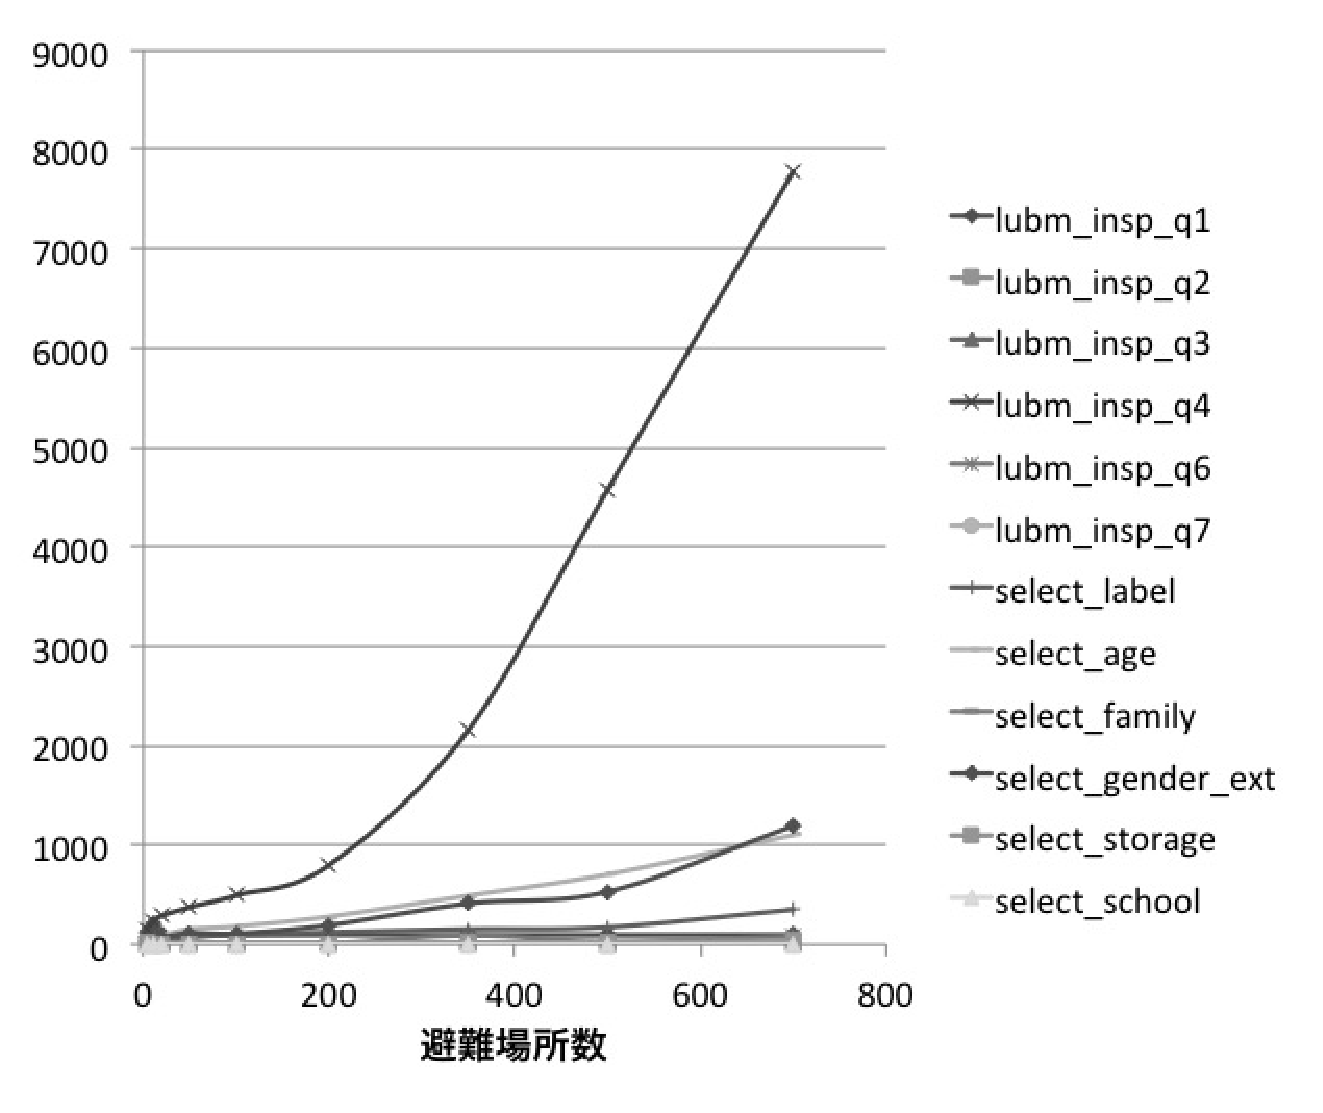
\includegraphics[width=120mm]{./images/test_query1.eps}
 		\caption{クエリ時間}
 		\label{fig:sibm_query_time}
 	\end{center}
\end{figure}

ここでは、避難場所数による時間がかかるクエリもあり、避難場所数に対する時間変動のないクエリもあると見える。

時間変動の多いクエリ(lubm\_insp\_q4、select\_label、select\_age、select\_gender\_ext)では、
クエリするデータの構造がより複雑であることがあり、または情報の条件に対する検索クエリである。

その一方、他のクエリでは、階層構成を持たないデータ(学校の情報など)や、検索条件が単純であるクエリの場合に対して、
時間変動がほとんどない、または少ないとわかる。

また、Jena/TDBを使用する時、数百避難場所の情報から検索すると、時間がかかることが見える。本実験の実験環境が最適化されていない原因や、
情報の構成の最適化を行ってないなどの理由が考えられるが、日本大震災の時、2500避難場所まで使用することがあり、またはより複雑な使用シナリオもあるため、
緊急時期で検索することで時間かかることは非常に影響があるだと考えられる。その際、従来の災害情報管理システムの設計に応じる問題となるかもしれない。
